\documentclass{article}
\usepackage[utf8]{inputenc}
\usepackage[english]{babel}
\usepackage{graphicx}
\usepackage{enumerate}
\usepackage{float}
\graphicspath{ {} }
\usepackage{mathtools}
\usepackage{amsmath, amsthm, amssymb, amsfonts}
\usepackage{caption}
\usepackage{fancyhdr}
\pagestyle{fancy}
\fancyhf{}
\rhead{Ty Darnell}
\lhead{663 Homework 2}

% For derivatives
\newcommand{\deriv}[1]{\frac{\mathrm{d}}{\mathrm{d}x} (#1)}

% For partial derivatives
\newcommand{\pderiv}[2]{\frac{\partial}{\partial #1} (#2)}

% Integral dx
\newcommand{\dx}{\mathrm{d}x}

\newcommand{\B}{\beta}

\allowdisplaybreaks
\begin{document}
\begin{flushleft}

	\section*{Problem 1}
\begin{enumerate}[(i)]
\item 
\begin{multline*}\\
X^{'}X=\left[
\begin{array}{rrrr}
1.00 & 1.00 & 1.00 & 1.00 \\ 
1.00 & 1.00 & 0.50 & 2.00 \\ 
\end{array}
\right]
\left[
\begin{array}{rr}
1.00 & 1.00 \\ 
1.00 & 1.00 \\ 
1.00 & 0.50 \\ 
1.00 & 2.00 \\ 
\end{array}
\right]=\left[
\begin{array}{rr}
4.00 & 4.50 \\ 
4.50 & 6.25 \\ 
\end{array}
\right]\\
(X^{'}X)^{-1}=\left[
\begin{array}{rr}
4.00 & 4.50 \\ 
4.50 & 6.25 \\ 
\end{array}
\right]^{-1}=\dfrac{1}{4.75}\left[\begin{array}{rr}
6.25 & -4.50 \\ 
-4.50 & 4 \\ 
\end{array}\right]=\left[
\begin{array}{rr}
1.315789 & -0.947368 \\ 
-0.947368 & 0.842105 \\ 
\end{array}
\right]\\
\end{multline*}

\item
\begin{multline*}\\
X^{'}Y=\left[
\begin{array}{rrrr}
1.00 & 1.00 & 1.00 & 1.00 \\ 
1.00 & 1.00 & 0.50 & 2.00 \\ 
\end{array}
\right]\left[
\begin{array}{r}
0.50 \\ 
-0.50 \\ 
0.30 \\ 
1.20 \\ 
\end{array}
\right]=\left[
\begin{array}{r}
1.50 \\ 
2.55 \\ 
\end{array}
\right]\\
\end{multline*}

\item
\begin{multline*}\\
\hat{\beta}=(X^{'}X)^{-1}X^{'}Y=\dfrac{1}{4.75}\left[\begin{array}{rr}
6.25 & -4.50 \\ 
-4.50 & 4 \\ 
\end{array}\right]\left[
\begin{array}{r}
1.50 \\ 
2.55 \\ 
\end{array}
\right]=\dfrac{1}{4.75}\left[
\begin{array}{r}
-2.1 \\ 
3.45 \\ 
\end{array}\right]=\left[
\begin{array}{r}
-.4421 \\ 
.7263 \\ 
\end{array}\right]\\
\end{multline*}

\item
\begin{multline*}\\
\hat{y}=X\hat{\beta}=\left[
\begin{array}{rr}
1.00 & 1.00 \\ 
1.00 & 1.00 \\ 
1.00 & 0.50 \\ 
1.00 & 2.00 \\ 
\end{array}
\right]\left[
\begin{array}{r}
-.4421 \\ 
.7263 \\ 
\end{array}\right]=\left[
\begin{array}{r}
0.28421 \\ 
0.28421 \\ 
-0.07895 \\ 
1.01053 \\ 
\end{array}
\right]\\
\end{multline*}

\item
\begin{multline*}\\
\hat{\epsilon}=y-\hat{y}=\left[
\begin{array}{r}
0.50 \\ 
-0.50 \\ 
0.30 \\ 
1.20 \\ 
\end{array}
\right]-\left[
\begin{array}{r}
0.28421 \\ 
0.28421 \\ 
-0.07895 \\ 
1.01053 \\ 
\end{array}
\right]=\left[
\begin{array}{r}
0.21579 \\ 
-0.78421 \\ 
0.37895 \\ 
0.18947 \\ 
\end{array}
\right]\\
\end{multline*}

\end{enumerate}
	
	\section*{Problem 2}
\begin{enumerate}[(a)]
	
	\item 
\begin{multline*}\\
H_0:\theta=\left[\begin{array}{r}
\B_1-\B_2\\
\B_2-\B_3\\
\B_3-\B_4
\end{array}\right]=\left[\begin{array}{r}
0\\
0\\
0
\end{array}\right]=\theta_0\\
\theta_{3x1}=C_{3x5} \ \B_{5x1}\\
\left[\begin{array}{r}
\B_1-\B_2\\
\B_2-\B_3\\
\B_3-\B_4
\end{array}\right]=C_{3x5} \left[\begin{array}{r}
\B_0\\
\B_1\\
\B_2\\
\B_3\\
\B_4
\end{array}\right]\\
C=\left[\begin{array}{rrrrr}
0&1&-1&0&0\\
0&0&1&-1&0\\
0&0&0&1&-1
\end{array}\right]\\
\left[\begin{array}{rrrrr}
0&1&-1&0&0\\
0&0&1&-1&0\\
0&0&0&1&-1
\end{array}\right]\left[\begin{array}{r}
\B_0\\
\B_1\\
\B_2\\
\B_3\\
\B_4
\end{array}\right]=\left[\begin{array}{r}
\B_1-\B_2\\
\B_2-\B_3\\
\B_3-\B_4
\end{array}\right]\\
\end{multline*}

	\item 
\begin{multline*}\\
H_0:\theta=\left[\begin{array}{r}
\B_1-\B_2\\
\B_3-\B_4
\end{array}\right]=\left[\begin{array}{r}
2\\
0
\end{array}\right]=\theta_0\\
\theta_{2x1}=C_{2x5} \ \B_{5x1}\\
\left[\begin{array}{r}
\B_1-\B_2\\
\B_3-\B_4
\end{array}\right]=C_{2x5}\left[\begin{array}{r}
\B_0\\
\B_1\\
\B_2\\
\B_3\\
\B_4
\end{array}\right]\\
C=\left[\begin{array}{rrrrr}
0&1&-1&0&0\\
0&0&0&1&-1
\end{array}\right]\\
\left[\begin{array}{rrrrr}
0&1&-1&0&0\\
0&0&0&1&-1
\end{array}\right]\left[\begin{array}{r}
\B_0\\
\B_1\\
\B_2\\
\B_3\\
\B_4
\end{array}\right]=\left[\begin{array}{r}
\B_1-\B_2\\
\B_3-\B_4
\end{array}\right]\\
\end{multline*}

	\item 
\begin{multline*}\\
H_0: \theta=\left[\begin{array}{r}
\B_1-2\B_2-4\B_3\\
\B_1+2\B_2
\end{array}\right]=\left[\begin{array}{r}
0\\
-6
\end{array}\right]=\theta_0\\
\theta_{2x1}=C_{2x5} \ \B_{5x1}\\
\left[\begin{array}{r}
\B_1-2\B_2-4\B_3\\
\B_1+2\B_2
\end{array}\right]=C_{2x5}\left[\begin{array}{r}
\B_0\\
\B_1\\
\B_2\\
\B_3\\
\B_4
\end{array}\right]\\
C=\left[\begin{array}{rrrrr}
0&1&-2&-4&0\\
0&1&2&0&0
\end{array}\right]\\
\left[\begin{array}{rrrrr}
0&1&-2&-4&0\\
0&1&2&0&0
\end{array}\right]\left[\begin{array}{r}
\B_0\\
\B_1\\
\B_2\\
\B_3\\
\B_4
\end{array}\right]=\left[\begin{array}{r}
\B_1-2\B_2-4\B_3\\
\B_1+2\B_2
\end{array}\right]\\
\end{multline*}
	
\end{enumerate}
\pagebreak
	\section*{Problem 3}
	
\begin{enumerate}[(a)]
	\item 
\begin{multline*}\\
\text{Looking at the reduced echelon form of X we have:}\\
\left[
\begin{array}{rrr}
1 & 0 & -1 \\ 
0 & 1 & 1 \\ 
0 & 0 & 0 \\ 
0 & 0 & 0 \\ 
0 & 0 & 0 \\ 
\end{array}
\right]\\
\text{The rank of X is 2 since we only have two non-zero rows.}\\
\text{Therefore X is not full rank and thus }\\
 \B \text{ is not estimable, but as many as 2 elements may be.} \\
\theta_1=\B_2=C_{1x3}\left[\begin{array}{r}
\B_0\\
\B_1\\
\B_2\\
\end{array}\right]\\
C=\left[\begin{array}{rrr}
0 & 0 &1
\end{array}\right]\\
\theta_i=C\beta =\B_2\\
\theta_1 \text{ is estimable } \iff C\beta= t^{'}_{1x5} \ E(y_{5x1})\\
E(y_{5x1})=X\beta=\left[\begin{array}{r}
\B_0+\B_1\\
\B_0+\B_1\\
\B_0-\B_2\\
\B_0-\B_2\\
\B_0+\B_1
\end{array}\right]\\
t^{'}_{1x5} \ E(y_{5x1})=\left[\begin{array}{rrrrr}
t_1&t_2&t_3&t_4&t_5
\end{array}\right]
\left[\begin{array}{r}
\B_0+\B_1\\
\B_0+\B_1\\
\B_0-\B_2\\
\B_0-\B_2\\
\B_0+\B_1
\end{array}\right]\\=\left[(t_1+t_2+t_5)(\B_0+\B_1)+(t_3+t_4)(\B_0-\B_2) \right]\\
\text{Since we cannot obtain } \B_2 \text{ from the result, it is not estimable}\\  
\end{multline*}

\pagebreak

	\item 
\begin{multline*}\\
\theta_2=\left[\begin{array}{r}
\B_0+\B_1\\
\B_0-\B_2
\end{array}\right]\\
t^{'}_{2x5} \ E(y_{5x1})=\left[\begin{array}{rrrrr}
t_{11}&t_{12}&t_{13}&t_{14}&t_{15}\\
t_{21}&t_{22}&t_{23}&t_{24}&t_{25}\\
\end{array}\right]\left[\begin{array}{r}
\B_0+\B_1\\
\B_0+\B_1\\
\B_0-\B_2\\
\B_0-\B_2\\
\B_0+\B_1
\end{array}\right]=\\
\left[\begin{array}{r}
(t_{11}+t_{12}+t_{15})(\B_0+\B_1)+(t_{13}+t_{14})(\B_0-\B_2)\\
(t_{21}+t_{22}+t_{25})(\B_0+\B_1)+(t_{23}+t_{24})(\B_0-\B_2\end{array} \right]\\
t^{'}_{2x5}=\left[\begin{array}{rrrrr}
1&0&0&0&0\\
0&0&1&0&0
\end{array}\right] \text{ is a solution}\\
\text{Thus } \theta_2 \text{ is estimable}\\
C=\left[\begin{array}{rrr}
1&1&0\\
1&0&-1
\end{array}\right]\\
\theta_2 \text{  testable since C is full rank and } \theta_2 \text{ is estimable}\\
\end{multline*}

\end{enumerate}

	\section*{Problem 4}
	
\begin{enumerate}[(a)]
	
	\item 	
\begin{tabular}{l|l|l|l|l|l}
\hline
Source&DF  &Sum of Squares  & Mean Square  & F Value & $Pr>F$  \\
\hline
Model&1  &2624.670184  &2624.670184  &137.906162& $\approx 0$ \\
\hline
Error& 96 & 1827.099916  & 19.0322908 &  \\
\hline
Corrected Total&97  &4451.7701  &  & \\
\hline
\end{tabular}
\begin{multline*}\\
MST=\dfrac{SSH}{DFH} \quad MSE=\dfrac{SSE}{DFE} \quad F=\dfrac{MSH}{MSE}\\
Pr>F =1-pf(137.906162,1,96)=0 \quad \text{(using R)}\\
\end{multline*}

	\item 
The model assumptions are:\\
Homogeneity of variance- every element of $\epsilon$ (error terms) has the same variance\\
Independence- each element of $\epsilon$ is independent of all others\\
Linearity- expected values of WGHT are linear function of the parameters. $E(y)=X\beta$\\
Existence - $\epsilon_i$ has finite first and second moments.\\
Gaussian errors- error terms are normally distributed. $\epsilon_i \sim N(0,\sigma_i^2)$\\

	\item 
$H_0:\B_1=0$\\
Since the p-value is approximately 0, reject the null hypothesis and conclude that average daily exercise time is a significant predictor of weight loss. \\

\end{enumerate}

	\section*{Problem 5}
\begin{enumerate}[(a)]
	
	\item 
$y=\B_0+\B_1X$\\
y=days x=index\\
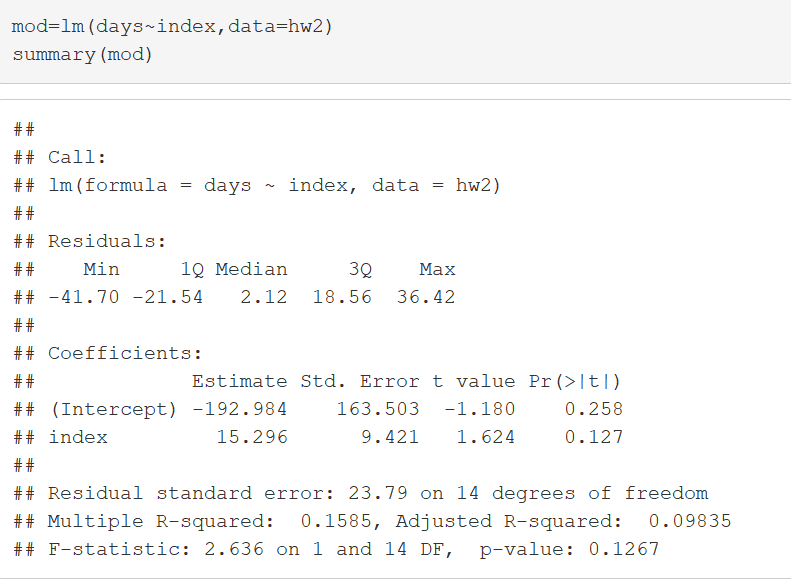
\includegraphics[scale=.8]{mod.png}\\
$\B_0$: When index = 0 the model predicts -192.984 high ozone days with a standard error of 163.503.\\
$\B_1$: with each increase of 1 in index, the model predicts an increase in 15.296 high ozone days with a standard error of 9.421. 
	\item 
Since X is full rank, all of the $\B$s are estimable\\
\pagebreak	
	\item 
$H_0:\B_1=0$\\
$\alpha=.05$\\
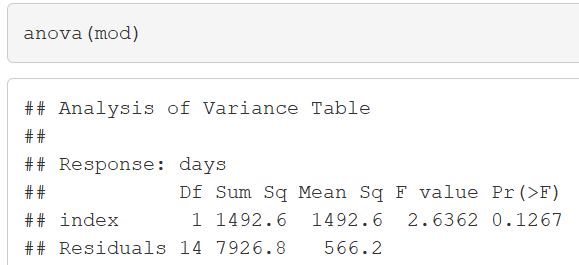
\includegraphics[scale=.7]{anova.png}\\
p-value=.1267\\
Conclusion: Fail to reject $H_0$ since p-value $>\alpha$\\
Thus we cannot conclude that the number high ozone days is associated with the meteorological index.
	\item 
\begin{multline*}\\
\alpha=.05\\
\text{t-statistic}=\dfrac{\hat{\B_1}-12}{SE_{\hat{\B_1}}}=(15.296-12)/9.421=.35\\
\text{p-value}=(1-pt(.35,14))*2=.7315\\
\text{Conclusion: fail to reject } H_0 \text{ since p-value}>\alpha\\
\text{We cannot conclude that a 1 degree increase in avg temp is associated}\\
\text{with a 12 day increase in number of high ozone days}\\
\end{multline*}

	\item 
95\% CI for expected number of high ozone days when index=16\\
$(21.76,81,76)$\\
95\% Prediction Interval for expected number of high ozone days when index=16\\
$(-7.44,110.96)$\\
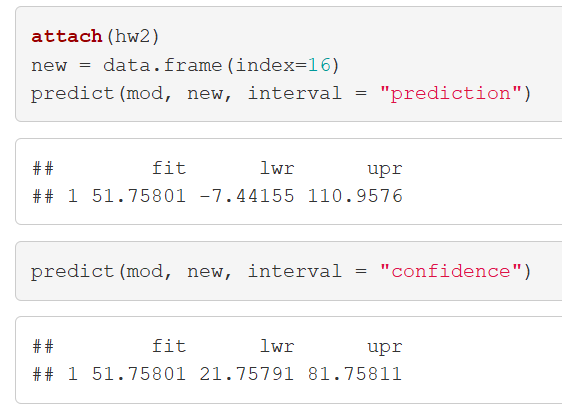
\includegraphics[scale=.7]{conf.png}\\
\end{enumerate}

\end{flushleft}
\end{document}
